In the previous section, we discussed the background of algebraic effects and handlers as developed by Plotkin, Pretnar and Power \cite{DBLP:journals/acs/PlotkinP03, DBLP:conf/lics/PlotkinP08}. The system has been worked out and has been implemented as the Eff programming language of which the calculus has been described in the previous section. This was the first language to have effects as first class citizens \cite{pretnar2015introduction}. Algebraic effects and handlers aren't just a fancy new concept, it is quickly maturing. There is more and more adoption of algebraic effects as a practical language feature for user-defined side-effects. As language features are being adopted more and more, optimization becomes a bigger priority.

This section is a summerization of the work by Matija Pretnar et al. of which I was a co-author. This work focusses on the optimization of algebraic effect and handlers. First, we explain why optimizations of algebraic effects and handlers are needed. Afterwards, the actual optimization and its evaluation is given. Finally, some issues with the optimizations are given. The novelty of my thesis, while not being a solution to these issues, arises from the work done in the optimizations.

\subsection{Motivation}

Considering that multiple implementation are available, runtime performance becomes much more important. Some implementations take the form a interpreters \cite{programming, links2ocaml}. Most implementations take the form of libraries \cite{DBLP:conf/icfp/Brady13, kammar, eff2ocaml}. Most work has been towards the optimization of the runtime performance. However, in the case of Eff, there still was a performance difference of about 4400\% between the algebraic effects and hand-written code in OCaml (without algebraic effects).

Another viable option was to provide an optimised compiler in order to transform the algebraic effects and handlers such that the runtime cost is avoided entirely \cite{optimization}. The optimised compiler is implemented for the Eff programming language. This work is one of the main driving factors behind the start of this thesis. 

The optimised compiler shows a lot of promise. By the end of this chapter, it will be clear that compile-time optimization is a very viable method of optimizing algebraic effects and handlers. However, there are some issues with this work, as wil be further discussed in Chapter~\ref{problems-eff}. More specifically, there are issues with the underlying type system of \eff. There are several methods of solving these issues, one of which leads to the work proposed in this thesis.

\subsection{Implementation}
There are two main ways that the optimising compiler used in order to optimise \eff code. The first is through the use of term rewriting rules, the other way is through purity aware compilation. Purity aware compilation provides a way for pure computations to have a more efficient representation, compared to the free monad representation. 

The term rewriting rules that were created during the creation of the optimised compiler is given in figure~\ref{fig:rewriterules}. These rules show how terms are rewritten in order to minimize the footprint of algebraic effects and handlers.

\begin{figure}
\begin{center}
\framebox{
\begin{minipage}{0.95\columnwidth}
\textbf{Simplification}\\
\begin{mathpar}
  \inferrule[App-Fun]{
% \textit{inlinable}(x, e ,c)
  }{
    (\fun{x} c) \, v \leadsto c [v/x]
  }

  \inferrule[Do-Ret]{
% \textit{inlinable}(x, e ,c)
  }{
    \doin{x \leftarrow \ret v} c \leadsto c [v / x]
  }


  \inferrule[Do-Op]{
  }{
    \doin{x \leftarrow (\doin{ y \leftarrow \op \,v } c_1 )} c_2 
    \quad\leadsto\quad
    \doin{y \leftarrow \op \,v} (\doin{x \leftarrow c_1} c_2)
  }

\end{mathpar}
\textbf{Handler Reduction}
\begin{mathpar}
  \inferrule[With-LetRec]{
  }{
    \withhandle{v}{(\letrecin{f \, x = c_1} c_2)} \leadsto
    \letrecin{f \, x = c_1} (\withhandle{v}{c_2}) 
  }

  \inferrule[With-Ret]{
    h = \shorthand
  }{
    \withhandle{h}{(\ret v)} \leadsto c_r[v/x]
  }

  \inferrule[With-Handled-Op]{
  \begin{array}{lr}
    h = \shorthand
  \end{array}
  }{
    \withhandle{h}{(\op \, v)} \leadsto
    c_\op[v / x, (\fun{x} c_r) / k]
  }

  \inferrule[With-Pure]{
     h = \shorthand \\
     \Gamma \vdash c : A \E \dirt \\
     \dirt \cap \ops = \emptyset
  }{
    \withhandle{h}{c} \leadsto \doin{x \leftarrow c} c_r
  }

  \inferrule[With-Do]{
    h = \shorthand \\
    h' = \shorthand[\ret y \mapsto (\withhandle{h}{c_2})]
  }
    {
    \withhandle{h}{(\doin{y \leftarrow c_1} c_2)} \leadsto
    \withhandle{h'}{c_1}
  }
\end{mathpar}
\end{minipage}
}
\end{center}

\caption{Term Rewriting Rules \cite{optimization}}\label{fig:rewriterules}
\end{figure}

There is also function specialisation, which is a special term rewrite rule. Function specialisation is used in order to deal with seemingly non-terminating recursive functions. Any recursive function \texttt{let rec f x = cf in c} that is used (and handled) can be rewritten with the following rewrite rule: \texttt{handle f v with h $\mapsto$ let rec f' x = handle cf with h in f' v}. In other words, function specialisation is about bringing handlers inside the function definition.

The standard way to compile algebraic effect handlers with free monad representations introduces a substantial performance overhead. This is especially the case for pure computations. We want to be able to differentiate between pure and impure computations.

One important aspect are the subtyping judgements that are used to elaborate types into functions that coerce one type into another, as seen in Figure~\ref{fig:elaboration:sub}. The elaboration judgement $(\ctx \ent v : A) \leadsto E$ and $(\ctx \ent c : \C) \leadsto E$ means that any value $v$ or any computation $c$ is elaborated into an \ocaml expression $E$. The different elaboration judgements can be seen in Figure~\ref{fig:elaboration:ext} and Figure~\ref{fig:elaboration:ext:c}. Note that the rules \textsc{SubVal} and \textsc{SubComp} utilise the subtyping judgements. The rules \textsc{HandPure}, \textsc{HandImpure}, \textsc{DoPure} and \textsc{DoImpure} distinguish between pure and impure cases in order to generate the most optimal code. A pure
$\ret v$ computation is translated just like the value $v$.

\begin{figure}
\begin{center}
\framebox{
\begin{minipage}{0.95\columnwidth}
\begin{mathpar}
  \inferrule[Sub-$\boolty$]{
  }{
    (\boolty \le \boolty) \leadsto (\fun{x}\,x)
  }

  \inferrule[Sub-$\intty$]{
  }{
    (\intty \le \intty) \leadsto (\fun{x}\,x)
  }

  \inferrule[Sub-$\to$]{
    (A' \le A) \leadsto E_1 \\
    (\C \le \C') \leadsto E_2 
  }{
    (A \to \C \le A' \to \C') \leadsto (\fun{f\,x}\,E_2\,(f\,(E_1\,x)))
  }

  \inferrule[Sub-$\hto$]{
    (\C' \le \C) \leadsto E_1 \\
    (\D \le \D') \leadsto E_2 
  }{
    (\C \hto \D \le \C' \hto \D') \leadsto (\fun{h\,x}\,E_2\,(h\,(E_1\,x)))
  }

  \inferrule[Sub-$\E$-Pure]{
    (A \le A') \leadsto E 
  }{
    (A \E \emptyset \le A' \E \emptyset) \leadsto E
  }

  \inferrule[Sub-$\E$-PureImpure]{
    (A \le A') \leadsto E  \\
    \dirt' \neq \emptyset
  }{
    (A \E \emptyset \le A' \E \dirt') \leadsto (\fun{x}\,\kord{return}\,(E\,x))
  }

  \inferrule[Sub-$\E$-Impure]{
    (A \le A') \leadsto E  \\
    \dirt \subseteq \dirt' \\ \dirt \neq \emptyset
  }{
    (A \E \dirt \le A' \E \dirt') \leadsto 
    (\kord{fmap}\,E)
  }
\end{mathpar}
\end{minipage}
}
\end{center}
\caption{Subtyping induced coercions \cite{optimization}}\label{fig:elaboration:sub}
\end{figure}

\begin{figure}
\begin{center}
\framebox{
\begin{minipage}{0.95\columnwidth}
\textbf{Values}
\begin{mathpar}
  \inferrule[SubVal]{
    (\ctx \ent v \T A) \leadsto E_1 \\
    (A \le A') \leadsto E_2
  }{
    (\ctx \ent v \T A') \leadsto (E_2\,E_1)
  }

  \inferrule[Var]{
    (x \T A) \in \ctx
  }{
    (\ctx \ent x \T A) \leadsto x
  }

  \inferrule[Const]{
    (\const \T A) \in \sig
  }{
    (\ctx \ent \const \T A) \leadsto \const
  }

  \inferrule[Fun]{ 
    (\ctx, x \T A \ent c \T \C) \leadsto E
  }{
    (\ctx \ent \fun{x} c \T A \to \C) \leadsto (\fun{x}\,E)
  }

  \inferrule[HandPure]{
    (\ctx, x \T A \ent c_r \T B \E \emptyset) \leadsto E_r
  }{
    (\ctx \ent \handler{\ret x \mapsto c_r} \T A \E \emptyset \hto B \E \emptyset) \leadsto (\fun{x}\,E_r)
  }

  \inferrule[HandImpure]{
    (\ctx, x \T A \ent c_r \T B \E \dirt) \leadsto E_r \\
    \Big[
      (\op \T A_\op \to B_\op) \in \sig \qquad
      (\ctx, x \T A_\op, k \T B_\op \to B \E \dirt \ent c_\op \T B \E \dirt)
      \leadsto E_{\op}
    \Big]_{\op \in \ops} \\
    {E_i = \begin{cases}
      \fun{x \, k} \comp{c_{\op_i}} & \op_i \in \ops \\
      \fun{x \, k} \ocop_i x \ocamlbind k & \op_i \in \dirt - \ops \\
      \fun{x \, k} \kpre{assert} \kord{false} & \text{otherwise}
    \end{cases}}
  }{
    (\ctx \ent \shorthand \T A \E \dirt \cup \ops \hto B \E \dirt)
    \\ \leadsto \kpre{handler} \{
      \kord{return} = \fun{x} E_r; \ocop_1 = E_1; \dots; \ocop_n = E_n\}
    \}
  }

\end{mathpar}
\end{minipage}
}
\end{center}
\caption{Type-\&-effect-directed purity aware compilation for expressions \cite{optimization}}\label{fig:elaboration:ext}
\end{figure}

\begin{figure}
\begin{center}
\framebox{
\begin{minipage}{0.95\columnwidth}
\textbf{Computations}
\begin{mathpar}
  \inferrule[SubComp]{
    (\ctx \ent c \T \C) \leadsto E_1 \\
    (\C \le \C') \leadsto E_2
  }{
    (\ctx \ent c \T \C') \leadsto (E_2\,E_1)
  }

  \inferrule[App]{
    (\ctx \ent v_1 \T A \to \C) \leadsto E_1 \\
    (\ctx \ent v_2 \T A) \leadsto E_2
  }{
    (\ctx \ent v_1 \, v_2 \T \C) \leadsto (E_1\,E_2)
  }

 \inferrule[LetRec]{
    (\ctx, f \T A \to \C, x \T A \ent c_1 \T \C) \leadsto E_1 \\
    (\ctx, f \T A \to \C \ent c_2 \T \D) \leadsto E_2
  }{
    (\ctx \ent \letrecin{f \, x = c_1} c_2 \T \D) \leadsto
    (\letrecin{f\,x = E_1}\,E_2)
  }

  \inferrule[Ret]{
    (\ctx \ent v \T A) \leadsto E
  }{
    (\ctx \ent \ret v \T A \E \emptyset) \leadsto E 
  }

  \inferrule[Op]{
    (\op \T A \to B) \in \sig \\
    (\ctx \ent v \T A) \leadsto E
  }{
    (\ctx \ent \op \, v \T B \E \{\op\}) \leadsto (\ocop\,E)
  }

  \inferrule[DoPure]{
    (\ctx \ent c_1 \T A \E \emptyset) \leadsto E_1 \\
    (\ctx, x \T A \ent c_2 \T B \E \emptyset) \leadsto E_2
  }{
    (\ctx \ent \doin{x \leftarrow c_1} c_2 \T B \E \emptyset)
    \leadsto (\letin{x = E_1}\,E_2 )
  }

  \inferrule[DoImpure]{
    (\ctx \ent c_1 \T A \E \dirt) \leadsto E_1 \\
    (\ctx, x \T A \ent c_2 \T B \E \dirt) \leadsto E_2 \\ 
    \dirt \neq \emptyset
  }{
    (\ctx \ent \doin{x \leftarrow c_1} c_2 \T B \E \dirt )
    \leadsto (E_1 \ocamlbind \fun{x} E_2)
  }
  
  \inferrule[With]{
    (\ctx \ent v \T \C \hto \D) \leadsto E_1 \\
    (\ctx \ent c \T \C) \leadsto E_2
  }{
    (\ctx \ent \withhandle{v}{c} \T \D) \leadsto (E_1\,E_2)
  }

\end{mathpar}
\end{minipage}
}
\end{center}
\caption{Type-\&-effect-directed purity aware compilation for computations \cite{optimization}}\label{fig:elaboration:ext:c}
\end{figure}

The combination of the purity aware compilation and the term rewrite rules allows for near complete optimization. In principle, handlers are pushed as deep as possible within the program until they can either be removed due to them not being needed (e.g. handling a value, handling an effect that does not appear in the handler clause) or until they can be evaluated (handling an operation term that does appear in the handler clause). The purity aware compilation then makes sure that pure computations are efficiently translated to \ocaml.

\subsection{Evaluation}
The optimising compiler needs to be evaluated empirically with several testing programs. This happens in two stages. First the different compilation schemes are compared with hand-written \ocaml code. Secondly, the compiler is compared against different implementations of algebraic effects and handlers. All benchmarks were run on a MacBook Pro with an 2.5 GHz Intel Core I7 processor and 16 GB 1600 MHz DDR3 RAM running Mac OS 10.12.3. The evaluation of the system devised in this thesis, as will be discussed in Chapter~\ref{eval}, cannot be directly compared against the results from the evaluation discussed here. The evaluation of Chapter~\ref{eval} was run on the same system running Mac OS 10.13.4 instead of 10.12.3.

In the first evaluation, \eff is compared against \ocaml. Figure~\ref{fig:loops} shows the runtime of a simple loop example that was used for this evaluation. The loop example used is shown below in figure~\ref{lst:loop}. Four different variations were used in the evaluation. A \textit{Pure} version was used containing no side-effects, a \textit{Latent} version which contains an effect that is never called during the runtime, a \textit{Inc} version which uses a single effect to increment an implicit state and a \textit{State} version which is what figure~\ref{lst:loop} shows. The \textit{State} version uses two operations \textit{Get} and \textit{Put} in order to perform operations on an implicit state. 

The \textit{Native} result is the execution of handwritten \ocaml code. The \textit{Basic} version is \eff without optimizations, while \textit{Opt}, \textit{Pure} and \textit{PureOpt} respectively perform optimization, purity aware compilation and both. In order to obtain the resuls, the execution run for \textit{10,000} iterations.

\begin{figure}
\caption{Loop code testing program}
\label{lst:loop}
\begin{lstlisting}[language=Caml]
effect Get: unit -> int
effect Put: int -> unit

let rec loop_state n =
    if n = 0 then
        ()
    else
        (#Put ((#Get ()) + 1); loop_state (n - 1))

let state_handler = handler
| val y -> (fun x -> x)
| #Get () k -> (fun s -> k s s)
| #Put s' k -> (fun _ -> k () s')

let test_state n =
    (with state_handler handle loop_state n) 0
\end{lstlisting}
\end{figure}

Within the second evaluation, the \textit{N-Queens} problem was used. \eff with optimization and purity aware compilation was tested against three other implementations of algebraic effects and handlers. Multicore Ocaml, which provides support for algebraic effect and handlers within \ocaml, was used. Multicore Ocaml provides a very efficient way to store and run algebraic effects on runtime. However, using a continuation multiple times requires an expensive copying operation of the continuation \cite{ocaml}. The other systems are the Handlers in Action implementation \cite{kammar} and the Eff Directly in OCaml implementation \cite{eff2ocaml}. 

The results are quite promising as the performance of fully optimised \eff becomes very similar to native code without algebraic effects. Comparing the performance against other systems also shows that our approach is consistently the fastest. 

\begin{figure}[H]
\centering
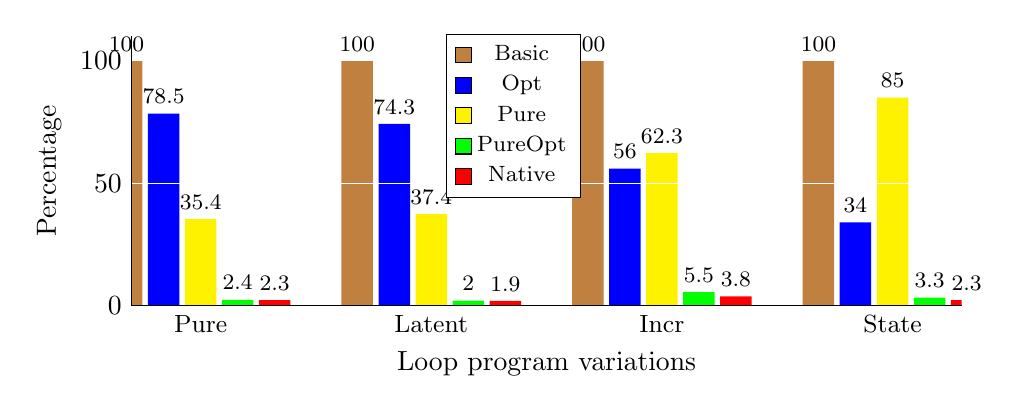
\begin{tikzpicture}
  \centering
  \begin{axis}[
        ybar, axis on top,
        height=5cm, width=\textwidth,
        ymajorgrids, tick align=inside,
        bar width=0.4cm,
        major grid style={draw=white},
        enlarge y limits={value=.1,upper},
        ymin=0, ymax=100,
        axis x line*=bottom,
        axis y line*=left,
        y axis line style={opacity=1},
        tickwidth=0pt,
        xtick = data,
        x tick label style={font=\small,text width=1.4cm,align=center},
         enlarge x limits=true,
      legend image code/.code={%
      \draw[#1] (0cm,-0.1cm) rectangle (0.2cm,0.1cm);
    },
            legend style={
            at={(0.46,1.01)},
            anchor=north,
            % legend columns=-1,
            % /tikz/every even column/.append style={column sep=0.4cm},
            font = \footnotesize
        },
        ylabel={Percentage},
        xlabel={Loop program variations},
           symbolic x coords={
           Pure,
           Latent,
           Incr,
           State,
           },
            nodes near coords={
         \footnotesize \pgfmathprintnumber{\pgfplotspointmeta}
        }
    ]
   \addplot [draw=none,fill=brown] coordinates {
      (Pure,100)
      (Latent,100)
      (Incr,100)
      (State,100)
       };

    \addplot [draw=none,fill=blue] coordinates {
      (Pure,78.5)
      (Latent,74.3)
      (Incr,56)
      (State,34)
      };

    \addplot [draw=none,fill=yellow] coordinates {
      (Pure,35.4)
      (Latent,37.4)
      (Incr,62.3)
      (State,85)
       };

    \addplot [draw=none,fill=green] coordinates {
      (Pure,2.4)
      (Latent,2)
      (Incr,5.5)
      (State,3.3)
       };

    \addplot [draw=none,fill=red] coordinates {
      (Pure,2.3)
      (Latent,1.9)
      (Incr,3.8)
      (State,2.3)
       }; 
   

    \legend{Basic, Opt, Pure, PureOpt, Native}
  \end{axis}
  \end{tikzpicture}
\caption{Relative run-times of Loops example \cite{optimization}}
\label{fig:loops}
\end{figure}

\begin{figure}[H]
  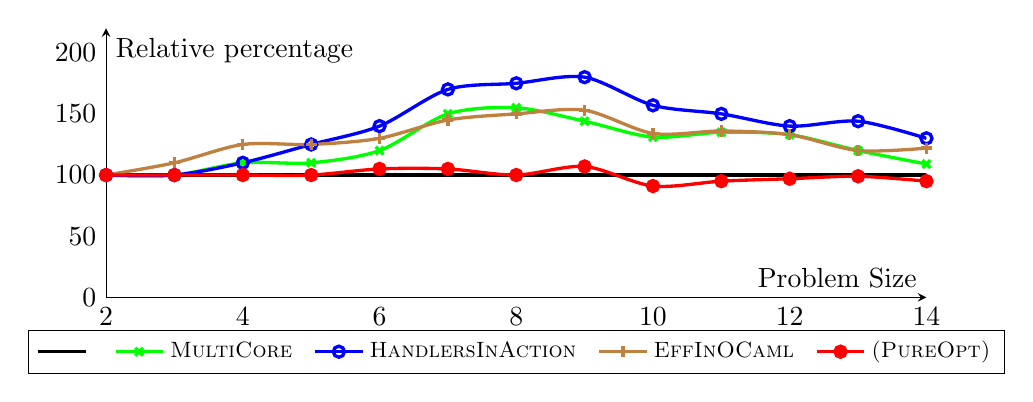
\begin{tikzpicture}
    \centering
    \begin{axis}[
          axis lines=center,
          axis on top,
          height=5cm, width=12cm,
          % bar width=0.4cm,
          % ymajorgrids, tick align=inside,
          major grid style={draw=white},
          enlarge y limits={value=.1,upper},
          ymin=0, ymax=200,
          axis x line*=bottom,
          axis y line*=left,
          % xtick = data,
          y axis line style={opacity=1},
          tickwidth=0pt,
          enlarge x limits=false,
          legend style={
              at={(0.5,-0.12)},
              anchor=north,
              legend columns=-1,
              /tikz/every even column/.append style={column sep=0.2cm},
              font = \footnotesize
          },
          ylabel={Relative percentage},
          xlabel={Problem Size},
             % symbolic x coords={
             % 0,
             % 8,
             % 9,
             % 10,
             % 11,
             % 12,
             % % 13,
             % % 14
             % },
         %      nodes near coords={
         %  \pgfmathprintnumber{\pgfplotspointmeta}
         % }
      ]
      %native
      \addplot [smooth,color = black, very thick] coordinates {
        (2,100)
        (3,100)
        (4,100)
        (5,100)
        (6,100)
        (7,100)
        (8,100)
        (9,100)
        (10,100)
        (11,100)
        (12,100)
        (13,100)
        (14,100)
         };
      %multicore
      \addplot [smooth,color = green, very thick, mark = x] coordinates {
        (2,100)
        (3,100)
        (4,110)
        (5,110)
        (6,120)
        (7,150)
        (8,155)
        (9,144)
        (10,131)
        (11,135)
        (12,133)
        (13,120)
        (14,109)
         };
      %HIA
     \addplot [smooth,color = blue, very thick, mark = o] coordinates {
        (2,100)
        (3,100)
        (4,110)
        (5,125)
        (6,140)
        (7,170)
        (8,175)
        (9,180)
        (10,157)
        (11,150)
        (12,140)
        (13,144)
        (14,130)
         };
      %EffectsinOcaml
     \addplot [smooth,color = brown, very thick, mark = +] coordinates {
        (2,100)
        (3,110)
        (4,125)
        (5,125)
        (6,130)
        (7,145)
        (8,150)
        (9,153)
        (10,134)
        (11,136)
        (12,133)
        (13,120)
        (14,122)
         };
      %PureOpt
     \addplot [smooth,color = red, very thick, mark = *] coordinates {
        (2,100)
        (3,100)
        (4,100)
        (5,100)
        (6,105)
        (7,105)
        (8,100)
        (9,107)
        (10,91)
        (11,95)
        (12,97)
        (13,99)
        (14,95)
         };
  
      \legend{\ocaml, \textsc{MultiCore}, \textsc{HandlersInAction}, \textsc{EffInOCaml}, \textsc{\eff}\textsc{(PureOpt)}}
    \end{axis}
    \end{tikzpicture}
  \caption{Results of running N-Queens for all solutions on multiple systems \cite{optimization}}
  \label{fig:systemsall}
  \end{figure}
  \begin{figure}[H]
  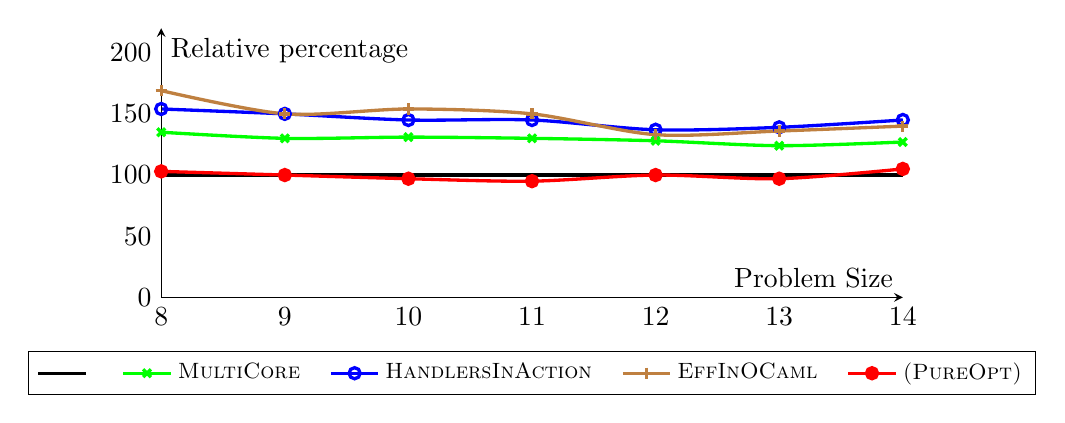
\begin{tikzpicture}
    \centering
    \begin{axis}[
          axis lines=center,
          axis on top,
          height=5cm, width=11cm,
          % bar width=0.4cm,
          % ymajorgrids, tick align=inside,
          major grid style={draw=white},
          enlarge y limits={value=.1,upper},
          ymin=0, ymax=200,
          axis x line*=bottom,
          axis y line*=left,
          xtick = data,
          y axis line style={opacity=1},
          tickwidth=0pt,
          enlarge x limits=false,
          legend style={
              at={(0.5,-0.2)},
              anchor=north,
              legend columns=-1,
              /tikz/every even column/.append style={column sep=0.3cm},
              font = \footnotesize
          },
          ylabel={Relative percentage},
          xlabel={Problem Size},
             % symbolic x coords={
             % 0,
             % 8,
             % 9,
             % 10,
             % 11,
             % 12,
             % % 13,
             % % 14
             % },
         %      nodes near coords={
         %  \pgfmathprintnumber{\pgfplotspointmeta}
         % }
      ]
      %native
      \addplot [smooth,color = black, very thick] coordinates {
        % (0,100)
        (8,100)
        (9,100)
        (10,100)
        (11,100)
        (12,100)
        (13,100)
        (14,100)
         };
      %multicore
      \addplot [smooth,color = green, very thick, mark = x] coordinates {
        (8,135)
        (9,130)
        (10,131)
        (11,130)
        (12,128)
        (13,124)
        (14,127)
         };
      %HIA
     \addplot [smooth,color = blue, very thick, mark = o] coordinates {
        (8,154)
        (9,150)
        (10,145)
        (11,145)
        (12,137)
        (13,139)
        (14,145)
         };
      %EffectsinOcaml
     \addplot [smooth,color = brown, very thick, mark = +] coordinates {
        (8,169)
        (9,150)
        (10,154)
        (11,150)
        (12,133)
        (13,136)
        (14,140)
         };
      %PureOpt
     \addplot [smooth,color = red, very thick, mark = *] coordinates {
        (8,103)
        (9,100)
        (10,97)
        (11,95)
        (12,100)
        (13,97)
        (14,105)
         };
  
      \legend{\ocaml, \textsc{MultiCore}, \textsc{HandlersInAction}, \textsc{EffInOCaml}, \textsc{\eff}\textsc{(PureOpt)}}
    \end{axis}
    \end{tikzpicture}
  \caption{Results of running N-Queens for one solution on multiple systems \cite{optimization}}
  \label{fig:systemsone}
  \end{figure}


\subsection{Limitations}\label{problems-eff}
As said in the motivation of this chapter, there are some issues with the optimizations. The main problem is that the optimising compiler of \eff is very fragile. The main reason is that the subtyping system is unclear to work with. With the implementation of \eff, every term is annotated with a type. This type also contains subtyping constraints. Term-rewrite rules work, as indicated by the name, with terms. Transforming most terms is easy. For example, under the right circumstances when \textsc{with-pure} is used, \texttt{handle c with h} is transformed into $\doin{x \leftarrow c} c_r$. The only change that occurs is the "shape" of the term, but the type remains the same.

This is not always the case. With function specialization, there is the rule \texttt{handle f v with h $\mapsto$ let rec f' x = handle cf with h in f' v}. With this term rewrite rule, a new recursive function \texttt{f'} needs to be created which is a specialization of the existing function \texttt{f}. Thus the type of \texttt{f'} needs to be correctly calculated. Calculating this type not only requires the types of the different terms, but also the subtyping constraints. It is quite easy to make mistakes and calculate the wrong type. With the wrong type, further optimizations might not be executed, or compilation might go completely wrong and cause typing errors. 

The main problem lies with the subtyping constraints and the implicit types of \eff. One possibility is to go to an explicitly typed calculus with Hindley-Milner based type inference. The effect system in such a system is based on row-typing \cite{type-directed, row, leijen2014koka}. Such an explicitly types calculus with row-based effects has been implemented in earlier research \cite{row-optimised}.  

Another possibility lies with a coercion-based system. This system is an explicitly-typed calculus for algebraic effects and handlers with support for subtyping using coercion proofs. This system uses coercion proofs in order to make the subtyping constraints an explicit element of the terms of the language. \cite{saleh2018explicit}

\subsection{Algebraic Subtyping}

When looking at different possibilities, we noticed the PhD thesis of Stephen Dolan. \cite{dolan2017algebraic}. Dolan provides a new subtyping based type system. While this system would not suffice for solving the issues with the optimizations, it does provide an interesting research direction for algebraic effects and handlers. 

Algebraic Subtyping has support for subtyping, but eliminates the disadvantage of having constraints. By using union and intersection types, subtyping constraints are explicitly coded within a type. For example, \lstinline{let twice f x = f (f x)} will be given the type: $(\beta \to \gamma) \to \alpha \to \gamma | \alpha \le \beta, \gamma \le \beta$. Algebraic subtyping will assign a different type to this term: $(\alpha \to \alpha \land \beta) \to \alpha \to \beta$. The two constraints are fully encoded within the type that the algebraic subtyping system infers. 

The advantage of utilising algebraic subtyping compared to subtyping is mainly the full elimination of the subtyping. This has the result that types become smaller in size and much more readable for users. Thus such a system would also be an advantage within the context of algebraic effects and handlers. 

The work in this thesis extends the algebraic subtyping system with algebraic effects and handlers. Chapter~\ref{core} explores the type system that algebraic subtyping provides and extends it in order to support algebraic effects and handlers. There will be clear mention of the novel elements, but the general guideline is that all algebraic effect and handler related work is novel, while the type system is not. 

Chapter~\ref{type-inference} extends the type inference algorithm from algebraic subtyping in order to support algebraic effects and handlers. The algorithm provided in the type inference chapter can infer very large types. These large types are not pleasent to look at and provide unnecessary overhead. Chapter~\ref{simplification} will extend simplification algorithms provided by the algebraic subtyping system. 

Chapter~\ref{implementation} provides information about the implementation and difficulties that were found. The implementation was done within the \eff programming language. Chapter~\ref{eval} evaluates the extended system using empirical evaluation. Correctness proofs have been added in Appendix~\ref{proofs}